\documentclass{article}

% if you need to pass options to natbib, use, e.g.:
%     \PassOptionsToPackage{numbers, compress}{natbib}
% before loading neurips_2026

% The authors should use one of these tracks.
% Before accepting by the NeurIPS conference, select one of the options below.
% 0. "default" for submission
\usepackage{neurips_2026}
% the "default" option is equal to the "main" option, which is used for the Main Track with double-blind reviewing.
% 1. "main" option is used for the Main Track
%  \usepackage[main]{neurips_2026}
% 2. "position" option is used for the Position Paper Track
%  \usepackage[position]{neurips_2026}
% 3. "eandd" option is used for the Evaluations & Datasets Track
 % \usepackage[eandd]{neurips_2026}
% 4. "creativeai" option is used for the Creative AI Track
%  \usepackage[creativeai]{neurips_2026}
% 5. "sglblindworkshop" option is used for the Workshop with single-blind reviewing
 % \usepackage[sglblindworkshop]{neurips_2026}
% 6. "dblblindworkshop" option is used for the Workshop with double-blind reviewing
%  \usepackage[dblblindworkshop]{neurips_2026}
% 7. "education" option is used for the Education Track
%  \usepackage[education]{neurips_2026}


% After being accepted, the authors should add "final" behind the track to compile a camera-ready version.
% 1. Main Track
 % \usepackage[main, final]{neurips_2026}
% 2. Position Paper Track
%  \usepackage[position, final]{neurips_2026}
% 3. Evaluations & Datasets Track
 % \usepackage[eandd, final]{neurips_2026}
% 4. Creative AI Track
%  \usepackage[creativeai, final]{neurips_2026}
% 5. Workshop with single-blind reviewing
%  \usepackage[sglblindworkshop, final]{neurips_2026}
% 6. Workshop with double-blind reviewing
%  \usepackage[dblblindworkshop, final]{neurips_2026}
% Note. For the workshop paper template, both \title{} and \workshoptitle{} are required, with the former indicating the paper title shown in the title and the latter indicating the workshop title displayed in the footnote.
% For workshops (5., 6.), the authors should add the name of the workshop, "\workshoptitle" command is used to set the workshop title.
% \workshoptitle{WORKSHOP TITLE}
% 7. Education Track
% \usepackage[education, final]{neurips_2026}

% "preprint" option is used for arXiv or other preprint submissions
 % \usepackage[preprint]{neurips_2026}

% to avoid loading the natbib package, add option nonatbib:
%    \usepackage[nonatbib]{neurips_2026}

\usepackage[utf8]{inputenc} % allow utf-8 input
\usepackage[T1]{fontenc}    % use 8-bit T1 fonts
\usepackage{hyperref}       % hyperlinks
\usepackage{url}            % simple URL typesetting
\usepackage{booktabs}       % professional-quality tables
\usepackage{amsfonts}       % blackboard math symbols
\usepackage{nicefrac}       % compact symbols for 1/2, etc.
\usepackage{microtype}      % microtypography
\usepackage{xcolor}         % colors

% Note. For the workshop paper template, both \title{} and \workshoptitle{} are required, with the former indicating the paper title shown in the title and the latter indicating the workshop title displayed in the footnote.

\usepackage{amsmath}
\usepackage{graphicx}
\newcommand{\todo}[1]{\textcolor{red}{[#1]}}

\title{Predicting Full-Benchmark LLM Accuracy from a Few Items: \\ Does Source-Model Data Beat Random Sampling?}

\author{Anonymous Authors}

\begin{document}

\maketitle

\begin{abstract}
Evaluating a language model on a full benchmark is expensive, so a growing literature selects a few items using the item-level results of existing (source) models and predicts the new (target) model's full accuracy from its answers to those items only. We ask when this source-model information actually beats the simplest practice, scoring a uniformly random subset. On 13 binary item-level score matrices (Open LLM Leaderboard v2 and HELM) we compare eleven selector--estimator pipelines under two protocols: a random split of models into sources and targets, and a capability-extrapolation split where the targets are the strongest 25\% of models. All methods see the same sources, targets and budgets ($n\le 200$ items), their hyperparameters never use target scores, and we report paired bootstrap intervals. On random splits every source-informed method has a lower macro-average MAE than the random subset mean at $n{=}50$ (4.6 accuracy points; 3.0--3.4 for the IRT, low-rank, supervised-selection and design-based pipelines, 3.7 for plain stratification, 4.3 for anchor points, which are no better than random from $n{=}100$), and rank correlation improves mostly at small $n$. Under extrapolation this advantage reverses for the methods that rely on a fitted model of the sources (MAE 6.5--8.1 points at $n{=}50$, worse than random) and their Spearman correlation drops from 0.64 to 0.46--0.56. What remains reliable is a design-based residual correction of the model's prediction (the difference estimator of survey sampling; ablations show that random items suffice and that it, not stratification, protects the model), and stratifying items by source difficulty when the estimate is the plain mean: they lower MAE by 0.7--1.6 points at $n{=}50$ in both regimes and are never significantly worse than random in any benchmark, split and budget, with intervals that also cover the choice of target models. The correction costs accuracy when targets resemble the sources, and its edge over plain stratification shrinks from about 1.5 points at $n{=}10$ to a third of a point at $n{=}50$. Source-model data thus help a lot when new models resemble the sources, only modestly otherwise, and no method recovers the ordering of models closer than a few accuracy points.
\end{abstract}

\section{Introduction}
\label{sec:intro}

Evaluating a language model on a benchmark means answering every item, and the cost multiplies when many checkpoints, prompts or inference settings are compared. A natural saving is to run the new model on a small subset of items and extrapolate to the full benchmark. Because per-item results of earlier models are routinely available, recent work uses them to choose the subset and to fit the extrapolation: clustering items into ``anchor points''~\citep{vivek2024anchor}, combining them with item response theory (IRT)~\citep{mauricio2024tiny,kipnis2025metabench}, or learning assessors and policies from earlier evaluations~\citep{pacchiardi2024100,li2025active}. These works report that tens to hundreds of items suffice, usually compared with random subsets.

The practical question is narrower than ``can few items predict the score''. A random subset already gives an unbiased estimate with a known standard error, $\sqrt{p(1-p)/n}$ up to a finite-population factor. Source models can help only by reducing variance or by encoding which items are informative, and they can hurt when the target differs from the sources, because a fitted model of the sources is then biased. We therefore ask, for binary item-level scores and at equal item budget $n\ll N$:
\begin{itemize}\setlength\itemsep{0pt}
\item[\textbf{Q1}] Does choosing items and fitting predictors with source-model data beat a random subset, in error (MAE, RMSE) and in ranking (Spearman, Kendall)?
\item[\textbf{Q2}] How does the answer change with the budget $n$, and how many items are needed for a given error?
\item[\textbf{Q3}] Does it survive when the target models are stronger than every source model?
\item[\textbf{Q4}] Is the error due to bias or to variance, and can models closer than the typical error be ranked?
\end{itemize}

\paragraph{Contributions.}
(i) A leakage-free comparison protocol on 13 public matrices in which every method gets identical sources, targets, budgets and seeds, hyperparameters are fixed in advance or chosen on source models only, and uncertainty is a paired bootstrap over seeds (Section~\ref{sec:setup}). (ii) Re-implementations of random, stratified, calibrated, anchor-point, IRT, low-rank and supervised-selection pipelines, plus a stratified design with a design-based residual correction (P3; the correction is the standard difference estimator of survey sampling, so P3 is a tested design rather than a new estimator) whose design was frozen by cross-validation inside the source models before the final run (Section~\ref{sec:methods}). (iii) The evidence that source-informed methods win clearly under random splits, that model-based ones lose to random sampling under extrapolation because of bias, and that designs with a design-based residual correction, and stratified sampling with the plain mean, are the only ones whose MAE is never significantly worse than random in our runs (also with intervals over target models), with a gain that is real but small; ablations show that the correction, not stratification, carries the robustness (Section~\ref{sec:exp}). The scope of these statements, which includes the implementation differences from the original methods, is stated in Section~\ref{sec:disc}.

\section{Related work}
\label{sec:related}

\paragraph{Choosing items from source-model results.}
Anchor Points~\citep{vivek2024anchor} cluster the response patterns of existing models and keep one representative item per cluster, estimating accuracy from these ``anchors''; the authors report that a handful of anchors can rank models better than a uniform random subset of the same size. tinyBenchmarks~\citep{mauricio2024tiny} combines such anchor items with item response theory (IRT) to estimate a new model's score, and reports that about a hundred curated MMLU items can suffice. metabench~\citep{kipnis2025metabench} selects items by IRT information fitted on a large population of models and reports reconstructing benchmark scores from under 3\% of the items. The learned-assessor approach of \citet{pacchiardi2024100} predicts a new model's success on unseen instances from its results on a few reference instances, and finds that random reference instances are close to more elaborate selection rules; their assessors use instance features, which are not available here. Active Evaluation Acquisition~\citep{li2025active} learns a policy that picks evaluation items adaptively, using a model of the dependencies between items to predict the remainder. We have read these works at the level of their abstracts and do not restate their protocols; the question our protocol is built around is whether the advantage over random sampling survives when the new model is stronger than all source models.

\paragraph{Benchmark-prediction evaluations.}
\citet{zhang2025benchmark} compare eleven benchmark-prediction methods on a collection of benchmarks and release the item-level score matrices and method implementations that we use as data (Section~\ref{sec:setup}). We use their data and, where stated, read their code, and we run every method ourselves under the protocol below; no number of theirs is reused.

\paragraph{Statistical background.}
Estimating a finite-population mean from a sample with the help of a model fitted on auxiliary information is the subject of model-assisted survey sampling~\citep{sarndal1992model}: stratified sampling uses auxiliary information in the design, and the difference (residual-correction) estimator adds to the model's population mean the sample mean of its residuals, which makes the estimator design-unbiased whatever the model. The same construction underlies prediction-powered inference~\citep{angelopoulos2023ppi}. Our P3 estimator (Section~\ref{sec:methods}) is this standard estimator with a low-rank model of the sources; we do not claim it as new, only test it as a design for benchmark prediction. Item response theory~\citep{embretson2000irt} is the latent-trait model on which the IRT pipelines are based. Adaptive evaluation with continuous scores~\citep{balkir2026confident}, which does not apply to binary item results, is outside our comparison. We also do not use sample-level benchmarking over open-ended capabilities~\citep{ghosh2024onebench}, since it is not a binary item matrix of the kind supplied; MMLU-Pro~\citep{wang2024mmlupro} enters only as one of the benchmarks of the Open LLM Leaderboard v2.

\paragraph{Benchmarks and score matrices.}
The Open LLM Leaderboard v2~\citep{fourrier2024openllm} and HELM~\citep{liang2023helm} provide the item-level correctness of many models on a common set of benchmarks, which is what makes source-model-based selection possible.

\section{Problem setting and evaluation protocol}
\label{sec:setup}

\paragraph{Setting.}
For a benchmark with $N$ items, let $M\in\{0,1\}^{K\times N}$ hold the correctness of $K$ models on every item. The models are partitioned into \emph{source} models $\mathcal S$, whose full rows are known, and \emph{target} models $\mathcal T$, which may be run on only $n\ll N$ items. A \emph{selector} chooses an item set $I$ with $|I|=n$ using $M_{\mathcal S}$ only (adaptive selectors may additionally use the target's answers already observed); a \emph{predictor} maps the target's outcomes on $I$ and $M_{\mathcal S}$ to an estimate $\hat y_t$ of the target's full accuracy $y_t=\frac1N\sum_i M_{ti}$. Target full scores are used only to score predictions; no selection, fitting or tuning step sees them. Hyperparameters are either fixed a priori (the IRT, low-rank and embedding sizes) or chosen on source models only (the ridge penalty and the design of P3, by cross-validation across source models); none is tuned on targets.

\paragraph{Metrics.}
For each benchmark, budget $n$ and split we report, over the target models, the mean absolute error (MAE) and root mean squared error (RMSE) of $\hat y_t$ against $y_t$ in percentage points of accuracy, and the Spearman and Kendall correlations between $\hat y$ and $y$.

\paragraph{Data.}
We use the item-level 0/1 score matrices of the benchmark-prediction repository of \citet{zhang2025benchmark} at the pinned commit \texttt{55faff4}, covering seven Open LLM Leaderboard v2 benchmarks and six HELM benchmarks (Table~\ref{tab:data}); model accuracies span a wide range, but are narrow for GPQA, MuSR and MATH Lvl5. ``Constant items'' are items on which all models agree; they are kept in $M$ and in $y_t$.

\begin{table}[t]
\caption{Score matrices used (model accuracies in \%). Generated by \texttt{figures/make\_data\_table.py}.}
\label{tab:data}
\centering\small
\begin{tabular}{lrrcr}
\toprule
Benchmark & Models & Items & Model accuracy (min / median / max) & Constant items \\
\midrule
IFEval & 448 & 541 & 3.7 / 27.8 / 88.0 & 1.3\% \\
BBH & 446 & 5761 & 24.1 / 44.2 / 74.7 & 0.0\% \\
GPQA & 447 & 1192 & 22.5 / 28.2 / 43.7 & 0.0\% \\
MuSR & 448 & 756 & 32.3 / 40.0 / 53.6 & 1.3\% \\
MATH Lvl5 & 447 & 894 & 0.0 / 2.1 / 35.6 & 13.3\% \\
MMLU-Pro & 448 & 12032 & 10.3 / 27.8 / 59.7 & 0.0\% \\
ARC-C & 218 & 1172 & 20.5 / 56.4 / 75.1 & 2.7\% \\
\midrule
HELM MMLU & 83 & 567 & 22.9 / 63.8 / 81.1 & 0.2\% \\
HELM GSM8K & 83 & 1000 & 2.8 / 73.4 / 95.6 & 0.3\% \\
HELM MATH & 83 & 437 & 2.5 / 65.0 / 93.4 & 0.2\% \\
HELM MedQA & 83 & 1000 & 21.5 / 61.0 / 86.9 & 0.2\% \\
HELM LegalBench & 79 & 2047 & 22.8 / 56.8 / 70.2 & 2.6\% \\
HELM Commonsense & 83 & 500 & 22.2 / 87.8 / 97.2 & 0.0\% \\
\bottomrule
\end{tabular}

\end{table}

\section{Methods compared}
\label{sec:methods}

Every method is a \emph{selector} (which $n$ items to run) plus an \emph{estimator} (how to turn the $n$ target answers into $\hat y$). Notation: $q_i$ is the mean accuracy of item $i$ over source models; $Y\in\{0,1\}^{|\mathcal T|\times n}$ are target answers on the selected items $I$.

\paragraph{Baselines without source models in the estimator.}
\textbf{B0} predicts the mean source accuracy and ignores the target's answers (a floor for MAE; it carries no ranking information). \textbf{B1} runs $n$ items drawn uniformly without replacement and predicts their mean; it is unbiased. \textbf{B2} sorts items by $q_i$, cuts them into $n$ equal strata, draws one item per stratum and predicts the mean; this uses the sources only to define strata, and keeps the design-based unbiasedness. \textbf{B3} takes the B1 subset mean and recalibrates it by a linear regression from subset mean to full accuracy fitted across source models.

\paragraph{Existing methods (our re-implementations).}
\textbf{Anchor points}~\citep{vivek2024anchor}: $k$-means with $k=n$ on a 16-dimensional SVD embedding of the item response vectors of the sources; the item nearest each centre is the anchor, and the prediction is the mean of the anchors weighted by cluster size. \textbf{Anchor+IRT} (in the spirit of~\citealp{mauricio2024tiny}): the same anchors, with a 4-dimensional two-parameter IRT model fitted on the sources, the target's ability estimated by MAP from its $n$ answers, and the prediction the mean predicted correctness probability over all items; no mixing with the anchor estimate. \textbf{Random+low-rank}: random items and a rank-8 latent-factor model of the sources whose target factors are estimated by MAP from the $n$ answers; the prediction is the mean of the completed row (a matrix-completion predictor related to~\citealp{pacchiardi2024100}, without item features). The IRT, low-rank and embedding sizes were fixed a priori and not tuned on targets.

\paragraph{Supervised selection (P1).}
\textbf{OMP+ridge}: greedy orthogonal matching pursuit chooses $n$ items whose responses best linearly reconstruct the source models' full accuracy; a ridge regression (penalty chosen by leave-one-out inside the sources) maps the target's answers on them to its full accuracy.

\paragraph{Further selectors and estimators (factorial analysis).}
The factorial analysis of Section~\ref{sec:exp} crosses six selectors with up to ten estimators: random, stratified, anchor, OMP, \emph{PPS} (inclusion probability proportional to the square root of the item's residual variance under the IRT fit of the sources) and a Bayesian \emph{c-optimal} design for the low-rank model, with the estimators mean, calibration, ridge, $k$-nearest-neighbour, IRT, low-rank, and IRT and low-rank with the residual correction.

\paragraph{Stratified design with a model-assisted correction (P3).}
Let $\hat p_{ti}\in[0,1]$ be the low-rank prediction for target $t$ on item $i$ given its $n$ answers. The estimator is $\hat y_t=\frac1N\sum_i \hat p_{ti}+\bar r_t$, where $\bar r_t$ is the inclusion-weighted mean residual $Y_{ti}-\hat p_{ti}$ over the selected items; with the stratified design (equal inclusion probabilities) this is the difference estimator of survey sampling, whose bias is controlled by the design and not by the model. We call it \textbf{P3 DR}. \textbf{P3 EB} shrinks the correction by $g=\bar r^2/(\bar r^2+\widehat{\mathrm{Var}}(\bar r))$, trusting the model more when the residual is within sampling noise. The selector, estimator and the two variants were chosen among 20 candidates (selectors random, stratified and two probability-proportional designs, with IRT or low-rank estimators and the two corrections, plus the baselines) by the lowest mean rank of MAE in an \emph{inner} cross-validation that treats part of the source models as targets and never touches the real targets (Section~\ref{sec:exp}); the frozen design is documented in \texttt{results/freeze/DESIGN\_FREEZE.md}. Ablations that use the same estimator with random items (\emph{random+low-rank+correction}), or the same stratified items with the plain model prediction (\emph{strat.+low-rank}), are reported in Section~\ref{sec:exp}.

\paragraph{Not implemented.}
Active Evaluation Acquisition~\citep{li2025active}, the metabench GAM predictor~\citep{kipnis2025metabench}, gp-IRT mixing and the Pacchiardi assessor with item features are not included; the last needs item text, which the matrices do not contain.

\section{Experiments}
\label{sec:exp}

\paragraph{Protocol.}
Per benchmark we draw 30 repetitions of two splits (Table~\ref{tab:data}). In the \emph{random} split a fresh 25\% of the models are targets and the rest are sources. In the \emph{extrapolation} split the targets are the strongest 25\% of models by full accuracy, so that every source is weaker than every target; the partition is deterministic, and its repetitions vary the selector seed and an 80\% subsample of the sources. Budgets are $n\in\{10,20,50,100,200\}$, capped at $N/4$ (so $n{=}200$ exists for 8 of 13 benchmarks, and macro-averages are shown for $n\le 100$, where all 13 benchmarks are present). Exact duplicate model rows are collapsed before splitting (Appendix~\ref{app:data}); the target accuracy is always the mean over all $N$ items. Seeds derive from a hash of (benchmark, split, repetition, $n$, selector), so every method sees identical splits. Per (benchmark, split, $n$, repetition) we compute the four metrics over the target models, and report means with 95\% percentile-bootstrap intervals over repetitions (1000 resamples; the macro curves, tables and per-benchmark figures); paired differences are taken within repetition. These intervals describe the noise of the selector and of the source subsample with the target models fixed, not the choice of the 20--107 target models of a benchmark. For the headline paired differences to B1 (macro and per benchmark, $n\in\{20,50,100\}$, both splits) we therefore use a two-level bootstrap: repetitions are resampled and then the target models within each resampled repetition, with identical indices for every method so that differences stay paired (1000 resamples; the macro interval treats the 13 benchmarks as fixed, and they share models, so it does not cover variation over benchmarks). Compared with the repetition-only intervals, these are $2$--$48$\% wider (median $12$\%) at $n{=}50$, and no conclusion changed. We write TB for them where the distinction matters. Macro-averages weight the 13 benchmarks equally; the benchmarks share models, so they are not independent, and cross-benchmark statements are descriptive. A random subset of $n$ items has RMSE equal to its analytic standard error to within sampling noise, and $n=N$ reproduces the exact score (sanity checks in \texttt{results/sanity/}).

\paragraph{Freezing P3.}
P3 was designed on 3 benchmarks (IFEval, GSM8K, MMLU-Pro) with an inner split made only of source models and then frozen (Section~\ref{sec:methods}); the exploration that preceded it (a few 2--4 seed pilot runs on GPQA and MMLU-Pro with outer targets, used to build the candidate list) and a disclosure about reading the data repository's README are listed in Appendix~\ref{app:honest}. P3 is therefore not tuned on the evaluated targets, but its independence is partial.

\subsection{Random split: source-model information helps}
Table~\ref{tab:macro} and Appendix Figure~\ref{fig:paired} (right) answer Q1 for random splits. At $n=50$ the macro MAE of the random subset mean (B1) is $4.60\pm0.13$ points, and every source-informed method has a paired MAE difference to B1 whose TB interval excludes zero on the macro-average (intervals in Table~\ref{tab:ablation}): $-0.30$ (anchor points), $-1.44$ (Anchor+IRT), $-1.27$ (OMP+ridge), $-1.50$ (random+low-rank), $-1.56$ (P3 EB), $-1.20$ (P3 DR), $-0.88$ (B2) points. The gains are not uniform: at $n{=}50$, whether a benchmark's TB interval lies below zero is true for Anchor+IRT on 10 of 13 benchmarks and OMP+ridge on 8, and OMP+ridge is worse on three HELM benchmarks (Commonsense, GSM8K, MATH; Table~\ref{tab:perbench}). The gain shrinks with $n$ (Anchor+IRT: $-4.57$ points at $n{=}10$, $-0.74$ at $n{=}100$) because a random subset catches up. Rank correlations behave alike: at $n{=}10$ OMP+ridge has Spearman $0.87$ against $0.67$ for B1; at $n{=}100$ all methods are within $0.04$ of each other (Table~\ref{tab:macro}, Appendix Figure~\ref{fig:paired}). Anchor points, as we implemented them, are the weakest of the source-informed family and exceed B1 in MAE at $n\ge100$ (+0.21 at $n{=}100$).

\begin{table}[t]
\caption{Macro-average over the 13 benchmarks of MAE (accuracy points) and Spearman correlation, mean $\pm$ half-width of the 95\% bootstrap interval over repetitions. Per-benchmark values in Appendix Table~\ref{tab:perbench}. Generated by \texttt{paper/make\_tables.py} from \texttt{figures/generated/}.}
\label{tab:macro}
\centering
{\scriptsize\setlength{\tabcolsep}{3pt}
\begin{tabular}{lrrrrrrrr}
\toprule
 & \multicolumn{3}{c}{MAE (points), random split} & \multicolumn{3}{c}{MAE (points), extrapolation} & \multicolumn{2}{c}{Spearman, $n{=}50$} \\
\cmidrule(lr){2-4}\cmidrule(lr){5-7}\cmidrule(lr){8-9}
Method & $n{=}20$ & $n{=}50$ & $n{=}100$ & $n{=}20$ & $n{=}50$ & $n{=}100$ & random & extrap. \\
\midrule
B0 mean of sources & 11.35\,{\tiny$\pm$0.13} & 11.35\,{\tiny$\pm$0.13} & 11.35\,{\tiny$\pm$0.12} & 21.32\,{\tiny$\pm$0.08} & 21.32\,{\tiny$\pm$0.08} & 21.32\,{\tiny$\pm$0.08} & -- & -- \\
B1 random & 7.45\,{\tiny$\pm$0.19} & 4.60\,{\tiny$\pm$0.13} & 3.18\,{\tiny$\pm$0.08} & 7.36\,{\tiny$\pm$0.26} & 4.54\,{\tiny$\pm$0.14} & 3.13\,{\tiny$\pm$0.12} & 0.85\,{\tiny$\pm$0.01} & 0.64\,{\tiny$\pm$0.01} \\
B2 stratified & 6.22\,{\tiny$\pm$0.10} & 3.72\,{\tiny$\pm$0.06} & 2.60\,{\tiny$\pm$0.04} & 6.13\,{\tiny$\pm$0.11} & 3.77\,{\tiny$\pm$0.08} & 2.59\,{\tiny$\pm$0.05} & 0.86\,{\tiny$\pm$0.01} & 0.67\,{\tiny$\pm$0.01} \\
B3 random + calibration & 4.89\,{\tiny$\pm$0.10} & 3.37\,{\tiny$\pm$0.05} & 2.42\,{\tiny$\pm$0.04} & 7.88\,{\tiny$\pm$0.22} & 5.11\,{\tiny$\pm$0.12} & 3.48\,{\tiny$\pm$0.10} & 0.85\,{\tiny$\pm$0.01} & 0.64\,{\tiny$\pm$0.01} \\
Anchor points & 6.47\,{\tiny$\pm$0.17} & 4.30\,{\tiny$\pm$0.12} & 3.39\,{\tiny$\pm$0.11} & 9.66\,{\tiny$\pm$0.23} & 6.85\,{\tiny$\pm$0.13} & 5.53\,{\tiny$\pm$0.10} & 0.87\,{\tiny$\pm$0.00} & 0.64\,{\tiny$\pm$0.01} \\
Anchor + IRT & 4.60\,{\tiny$\pm$0.07} & 3.16\,{\tiny$\pm$0.05} & 2.45\,{\tiny$\pm$0.05} & 9.97\,{\tiny$\pm$0.12} & 7.64\,{\tiny$\pm$0.08} & 6.52\,{\tiny$\pm$0.07} & 0.91\,{\tiny$\pm$0.00} & 0.56\,{\tiny$\pm$0.01} \\
Random + low-rank & 4.45\,{\tiny$\pm$0.08} & 3.10\,{\tiny$\pm$0.05} & 2.37\,{\tiny$\pm$0.04} & 9.62\,{\tiny$\pm$0.13} & 8.10\,{\tiny$\pm$0.08} & 7.33\,{\tiny$\pm$0.06} & 0.90\,{\tiny$\pm$0.00} & 0.46\,{\tiny$\pm$0.02} \\
P1 OMP + ridge & 3.66\,{\tiny$\pm$0.08} & 3.33\,{\tiny$\pm$0.08} & 2.28\,{\tiny$\pm$0.04} & 7.46\,{\tiny$\pm$0.11} & 6.45\,{\tiny$\pm$0.11} & 5.47\,{\tiny$\pm$0.08} & 0.91\,{\tiny$\pm$0.00} & 0.47\,{\tiny$\pm$0.02} \\
P3 DR (stratified + low-rank + correction) & 5.40\,{\tiny$\pm$0.09} & 3.40\,{\tiny$\pm$0.05} & 2.38\,{\tiny$\pm$0.03} & 5.51\,{\tiny$\pm$0.11} & 3.43\,{\tiny$\pm$0.06} & 2.45\,{\tiny$\pm$0.04} & 0.87\,{\tiny$\pm$0.00} & 0.67\,{\tiny$\pm$0.01} \\
P3 EB (shrunk correction) & 4.70\,{\tiny$\pm$0.08} & 3.04\,{\tiny$\pm$0.05} & 2.16\,{\tiny$\pm$0.03} & 5.97\,{\tiny$\pm$0.12} & 3.80\,{\tiny$\pm$0.08} & 2.71\,{\tiny$\pm$0.05} & 0.90\,{\tiny$\pm$0.00} & 0.67\,{\tiny$\pm$0.01} \\
\bottomrule
\end{tabular}}

\end{table}

\begin{figure}[t]
\centering
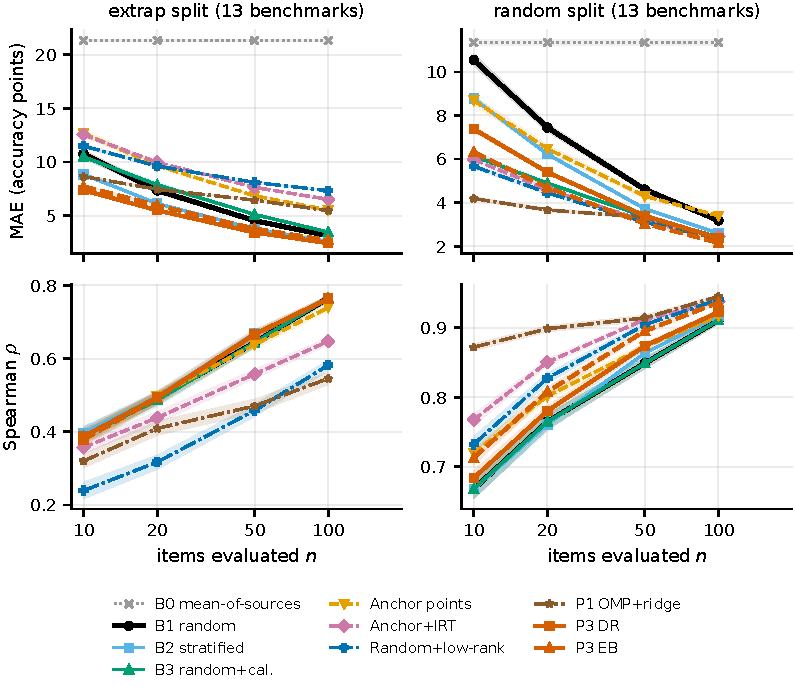
\includegraphics[width=0.8\linewidth]{../figures/generated/fig_macro_curves.pdf}
\caption{Macro-average over the 13 benchmarks of MAE (top) and Spearman correlation (bottom) against the number of items $n$ ($n\le100$), extrapolation split (left) and random split (right), 95\% bands over repetitions.}
\label{fig:macro}
\end{figure}

\subsection{Extrapolation: model-based predictors lose to random sampling}
When the targets are the strongest models, the picture changes (Table~\ref{tab:macro}, Appendix Figure~\ref{fig:paired} left). At $n=50$ the macro MAE of Anchor points, Anchor+IRT, random+low-rank and OMP+ridge is $6.85$, $7.64$, $8.10$ and $6.45$ points, against $4.54$ for B1; the paired differences are $+2.31$, $+3.10$, $+3.56$ and $+1.91$ points, and they are worse than B1 on 7, 11, 10 and 9 of 13 benchmarks. They stay worse as $n$ grows (random+low-rank: $+4.95$ at $n{=}200$). Their Spearman correlation drops to $0.46$--$0.64$ against $0.64$ for B1 and is below B1 by $0.09$--$0.19$ at $n{=}50$ for the three model-based methods. The scatter plots (Appendix Figure~\ref{fig:scatter}) show the cause: the strongest targets are predicted too low, a mean signed error of Anchor+IRT of $-12.2$ points for the targets in the top quartile of true accuracy within each benchmark and $-6.3$ for the others (pooled over benchmarks and repetitions; \texttt{figures/generated/fig\_scatter\_extrap\_bias.csv}), and, in terciles of the targets of each benchmark, $-5.0$, $-7.2$ and $-10.6$ (\texttt{q4\_by\_true\_tercile.csv}). Calibration (B3) also becomes worse than B1 ($+0.58$ points at $n{=}50$, interval $[0.39,0.77]$).

What survives is the design-based residual correction and, for the plain mean, stratification. Table~\ref{tab:ablation} separates the ingredients (13 benchmarks, TB intervals, $n{=}50$ unless stated). Without the correction the low-rank model is $+3.56$ points above B1 ($[3.37,3.74]$) with random items and $+3.54$ ($[3.35,3.73]$) with stratified items, so stratification does not protect it. Adding the correction brings it to $-0.99$ ($[-1.14,-0.83]$) with random items and $-1.10$ ($[-1.27,-0.94]$) with stratified items (P3 DR); the correction changes the MAE by $-4.55$ and $-4.65$ points. Stratification gives $-0.77$ ($[-0.95,-0.61]$) with the plain mean (B2), but given the correction only $-0.12$ ($[-0.20,-0.03]$) at $n{=}50$, and nothing distinguishable from zero at $n{=}20$ ($-0.01$, $[-0.18,0.15]$) and $n{=}100$ ($-0.04$, $[-0.10,0.02]$; these contrasts use repetition-only intervals). P3 EB, which shrinks the correction, is $0.36$ ($[0.32,0.40]$) worse than P3 DR under extrapolation and $0.36$ better on the random split. The robustness to extrapolation therefore comes from the correction, for which a random subset suffices, and stratification adds a gain mostly when the estimator is the plain mean; our earlier reading, that stratification carries P3's gain, is not supported. Against B2, P3 DR is better by $1.48$ points at $n{=}10$ (13 of 13 benchmarks; repetition-only intervals, since $n{=}10$ was not in the two-level bootstrap) but by only $0.33$ at $n{=}50$ (TB: below zero on 8 of 13 benchmarks, above on none) and $0.14$ at $n{=}100$ (6 of 13); P3 EB is not better than B2 under extrapolation at $n\ge50$ ($+0.03$, $[-0.07,0.11]$ at $n{=}50$ with 5 of 13 benchmarks worse; $+0.12$, $[0.06,0.18]$ at $n{=}100$). Against B1, none of B2, P3 DR, P3 EB or random+low-rank+correction has a TB interval above zero in any of the 78 cells (13 benchmarks $\times$ 2 splits $\times$ 3 budgets), so ``never significantly worse than B1'' holds; ``better on every benchmark'' does not: P3 DR has a TB interval below zero on 13 of 13 benchmarks at $n{=}50$ (both splits) and at $n{=}100$ on the random split, but on $10$--$12$ of 13 in the other cells (extrapolation: $11$, $13$ and $10$ at $n{=}20,50,100$; random: $12$, $13$, $13$); P3 EB on only $6$ of 13 at $n{=}50$ under extrapolation. The Spearman correlations of B2, P3 DR and P3 EB are $0.02$--$0.03$ above those of B1 at $n{=}50$ with TB intervals that reach zero for P3 DR and P3 EB (Appendix Table~\ref{tab:metrics}). So, on the extrapolation split, the source data buy a modest gain in error and nothing detectable in ranking, which answers Q1 and Q3; RMSE and Kendall give the same conclusions (Appendix Table~\ref{tab:metrics}).

\begin{table}[t]
\caption{Ablation of P3 on the 13 Tier-1 benchmarks: MAE difference to the random subset mean B1 (points; negative is better), with 95\% two-level (repetitions, then target models) bootstrap intervals, and contrasts between estimators (repetition-only intervals, same sign convention: first minus second). Generated by \texttt{paper/make\_tables.py} from \texttt{results/tables/review/}.}
\label{tab:ablation}
\centering
\resizebox{\linewidth}{!}{{\scriptsize\setlength{\tabcolsep}{2pt}
\begin{tabular}{lrrrrrr}
\toprule
 & \multicolumn{3}{c}{random split} & \multicolumn{3}{c}{extrapolation} \\
\cmidrule(lr){2-4}\cmidrule(lr){5-7}
Estimator (difference in MAE to B1, points) & $n{=}20$ & $n{=}50$ & $n{=}100$ & $n{=}20$ & $n{=}50$ & $n{=}100$ \\
\midrule
B2 stratified (plain mean) & -1.22\,{\tiny[-1.45,-0.99]} & -0.88\,{\tiny[-1.04,-0.73]} & -0.59\,{\tiny[-0.69,-0.48]} & -1.23\,{\tiny[-1.53,-0.92]} & -0.77\,{\tiny[-0.95,-0.61]} & -0.54\,{\tiny[-0.68,-0.42]} \\
Random + low-rank (no correction) & -3.00\,{\tiny[-3.19,-2.79]} & -1.50\,{\tiny[-1.64,-1.35]} & -0.82\,{\tiny[-0.92,-0.71]} & +2.26\,{\tiny[+1.94,+2.57]} & +3.56\,{\tiny[+3.37,+3.74]} & +4.20\,{\tiny[+4.06,+4.33]} \\
Random + low-rank + correction & -2.01\,{\tiny[-2.18,-1.82]} & -1.13\,{\tiny[-1.26,-0.99]} & -0.78\,{\tiny[-0.88,-0.70]} & -1.84\,{\tiny[-2.15,-1.56]} & -0.99\,{\tiny[-1.14,-0.83]} & -0.64\,{\tiny[-0.76,-0.52]} \\
Stratified + low-rank (no correction) & -3.07\,{\tiny[-3.29,-2.83]} & -1.54\,{\tiny[-1.70,-1.38]} & -0.82\,{\tiny[-0.93,-0.72]} & +2.31\,{\tiny[+2.01,+2.61]} & +3.54\,{\tiny[+3.35,+3.73]} & +4.18\,{\tiny[+4.03,+4.31]} \\
P3 DR (stratified + low-rank + correction) & -2.05\,{\tiny[-2.28,-1.81]} & -1.20\,{\tiny[-1.36,-1.05]} & -0.81\,{\tiny[-0.92,-0.71]} & -1.85\,{\tiny[-2.17,-1.55]} & -1.10\,{\tiny[-1.27,-0.94]} & -0.68\,{\tiny[-0.81,-0.55]} \\
P3 EB (shrunk correction) & -2.75\,{\tiny[-2.97,-2.52]} & -1.56\,{\tiny[-1.72,-1.40]} & -1.03\,{\tiny[-1.13,-0.93]} & -1.39\,{\tiny[-1.72,-1.08]} & -0.74\,{\tiny[-0.92,-0.58]} & -0.42\,{\tiny[-0.55,-0.28]} \\
\midrule
Contrast: DR correction, given random items & +0.99\,{\tiny[+0.93,+1.06]} & +0.37\,{\tiny[+0.32,+0.42]} & +0.03\,{\tiny[-0.01,+0.07]} & -4.10\,{\tiny[-4.24,-3.97]} & -4.55\,{\tiny[-4.64,-4.46]} & -4.84\,{\tiny[-4.91,-4.77]} \\
Contrast: DR correction, given stratified items & +1.02\,{\tiny[+0.95,+1.08]} & +0.34\,{\tiny[+0.29,+0.38]} & +0.01\,{\tiny[-0.02,+0.05]} & -4.16\,{\tiny[-4.28,-4.03]} & -4.65\,{\tiny[-4.72,-4.57]} & -4.86\,{\tiny[-4.92,-4.79]} \\
Contrast: stratification, given DR & -0.04\,{\tiny[-0.18,+0.09]} & -0.07\,{\tiny[-0.14,-0.01]} & -0.02\,{\tiny[-0.07,+0.03]} & -0.01\,{\tiny[-0.18,+0.15]} & -0.12\,{\tiny[-0.20,-0.03]} & -0.04\,{\tiny[-0.10,+0.02]} \\
Contrast: stratification, plain mean & -1.22\,{\tiny[-1.44,-1.02]} & -0.88\,{\tiny[-1.02,-0.76]} & -0.59\,{\tiny[-0.68,-0.50]} & -1.23\,{\tiny[-1.51,-0.94]} & -0.77\,{\tiny[-0.93,-0.61]} & -0.54\,{\tiny[-0.67,-0.42]} \\
Contrast: EB shrinkage vs DR & -0.70\,{\tiny[-0.73,-0.66]} & -0.36\,{\tiny[-0.38,-0.34]} & -0.22\,{\tiny[-0.24,-0.20]} & +0.46\,{\tiny[+0.40,+0.53]} & +0.36\,{\tiny[+0.32,+0.40]} & +0.26\,{\tiny[+0.23,+0.29]} \\
\bottomrule
\end{tabular}}
}
\end{table}

\subsection{Budget and items needed}
Error falls roughly as $1/\sqrt n$ for all unbiased designs (Figure~\ref{fig:curves} in the appendix). Interpolating the mean-MAE curves of each benchmark, the number of items needed to reach an MAE of $2$ points within the evaluated budgets ($n\le\min(200,N/4)$) is attained on the extrapolation split on only $4$ of 13 benchmarks for B1 (median $\approx 141$ items among them), $6$ for B2 (median $\approx 139$) and $7$ for P3 DR (median $\approx 129$); model-based methods reach it on $0$--$2$ benchmarks. On random splits, B1 reaches it on $2$ benchmarks, P3 EB on $10$ (median $\approx118$) and OMP+ridge on $6$ (median $\approx 22$ items; \texttt{results/tables/tier1/items\_needed.csv}). Hence a 2-point error needs on the order of a hundred items on many benchmarks, and in the extrapolation case it is not reached on most benchmarks within the cap $N/4$ (a limit of the grid, not a statement about larger budgets).

\subsection{Where the error comes from, and ranking}
For each target model we separate the squared bias of its prediction over repetitions from the variance over repetitions (Appendix Table~\ref{tab:q4}, $n{=}50$, mean over benchmarks and targets). Under extrapolation the IRT, low-rank and OMP methods have much lower variance ($3.8$--$7.3$ points$^2$) than B1 ($32.2$), but a squared bias of $58$--$88$ against B1's $1.2$, which is about the estimation floor for the extrapolation split (the variance of B1 divided by the $30$ draws is about $1.1$); anchor points have both a high bias ($109$) and a high variance ($23$). The design-based methods B2, P3 DR and P3 EB keep a squared bias of $0.7$--$5.9$ and cut the variance from $32.2$ to $17$--$23$. On random splits a model is a target in only about a quarter of the $30$ repetitions ($\approx7.5$ draws), so the floor for an unbiased design is about $4$ (B1: squared bias $5.1$, variance $29.9$); the squared bias is at most $14$ points$^2$ for every method but B0, and the model-based ones reduce the variance, which is why they win there.

Models closer than a few points are not ranked reliably by any method (Appendix Figure~\ref{fig:pairwise}, $n{=}50$): for pairs whose true accuracies differ by less than 1 point the fraction of correctly ordered pairs is $0.50$--$0.51$ for B1 and P3 DR in both splits, rising to $0.59$--$0.62$ for gaps of 1--2 points and to $0.71$--$0.73$ for 2--5 points on the extrapolation split; Anchor+IRT is mostly better than B1 on random splits, and Anchor+IRT and OMP+ridge are worse than B1 on the extrapolation split for gaps above 5 points. High macro rank correlations (Table~\ref{tab:macro}) therefore reflect the large spread of model accuracy and not the ability to resolve close models.

\subsection{Further analyses}
These analyses were run after the Tier-1 results and the design freeze, on subsets of the benchmarks (7 for the factorial, source-size and coverage analyses; 4 for the organisation hold-out; 5 for the rank ablation, chosen by the analysis owner for computing time) with 20 repetitions; none of them changed a Tier-1 number or the frozen P3 design. Intervals below are repetition-bootstrap intervals with fixed targets, like those above (appendix tables give the MAE values of every cell; the full tables with intervals are in \texttt{results/tables/macro/}).

\paragraph{Organisation hold-out behaves like the random split.}
We also held out all models of one organisation (the prefix of the model name; four folds, the four Open LLM Leaderboard benchmarks only, because the HELM model names carry no verifiable family label). The organisation prefix is a coarse family label, since community fine-tunes sit under other prefixes, and this split is not a capability shift. At $n{=}50$ the macro MAE on these four benchmarks is B1 $4.87$, B2 $4.20$, P3 DR $3.73$, random+low-rank $2.88$ and OMP+ridge $2.20$, almost the same as on the random split of the same benchmarks ($4.91$, $4.18$, $3.72$, $2.78$, $1.95$; Table~\ref{tab:family}) and unlike their extrapolation values ($5.21$, $4.61$, $4.18$, $10.04$, $7.16$). Across the twelve methods the Spearman correlation of their MAE between the random and the organisation hold-out split is $+0.97$ to $+1.00$ ($n{=}20,50,100$), and between the random and the extrapolation split $-0.51$ to $-0.62$: leaving out one organisation does not reproduce the reversal that leaving out the strongest models causes, so conclusions on interpolation do not transfer to capability shift.

\paragraph{Which ingredient protects against extrapolation.}
Table~\ref{tab:factorial} crosses selectors and estimators ($n{=}50$, 7 benchmarks, 20 repetitions). Under extrapolation every estimator that uses a fitted model of the sources without correction (ridge, $k$-NN, IRT, low-rank) has an MAE of $7.8$ to $12.5$ points with every selector, and calibration $5.4$ to $11.5$, against $4.65$ for random items with the subset mean. Adding the residual correction brings the same models to $3.9$--$4.1$ points with random, stratified and PPS items (random+low-rank+correction: $3.91$, paired difference to B1 $-0.74$ points, interval $[-0.88,-0.60]$; stratified+low-rank+correction $3.72$, $-0.93$, $[-1.11,-0.75]$). So the protection comes from the correction, and a random subset suffices for it; stratification, which alone gives $4.04$ with the mean ($-0.61$, $[-0.80,-0.40]$), adds a further $0.2$ points to the corrected model (a difference we did not test pairwise on this subset). The correction has a price when sources are informative: on the random split the plain low-rank model with stratified items has MAE $3.14$ and the corrected one $3.64$ (B1 $4.82$), and on all 13 Tier-1 benchmarks $3.06$ against $3.40$. Selectors that use the sources to look for informative items (OMP, c-optimal) are good only with a model estimator and are poor with the plain mean ($8.53$ and $14.91$ points on the random split), as their items are not representative of the benchmark. The Tier-1 ablations on all 13 benchmarks (Table~\ref{tab:ablation}) agree.

\paragraph{Number of source models.}
With few source models (Table~\ref{tab:ssize}; 7 benchmarks, $n{=}50$) the fitted models lose their advantage on the random split: random+low-rank has an MAE of $5.38$, $4.43$ and $3.64$ with $10$, $20$ and $40$ source models and $3.18$ with all, against $4.82$ for B1 (which does not use the sources); Anchor+IRT is at $8.08$ with $10$ sources. P3 DR is at $4.15$, $4.00$, $3.87$ and $3.63$ and P3 EB at $3.94$, $3.69$, $3.46$ and $3.18$, so the design-based methods are not worse than B1 even with $10$ sources. Under extrapolation more sources do not remove the bias of the model-only estimators ($14.24$ to $9.85$ for random+low-rank) while P3 DR stays at $4.26$--$3.75$ against $4.65$ for B1.

\paragraph{Sensitivity to the rank of the latent model.}
We varied the rank $k\in\{2,4,8,16,32\}$ of the low-rank model in the stratified designs (5 benchmarks, $n{=}50$, Table~\ref{tab:rank}; $k{=}8$ is the frozen P3 and was fixed before the results). Under extrapolation P3 DR is between $3.55$ and $3.74$ points for $k\le16$ (B1: $4.36$ on these benchmarks) and worse than B1 at $k{=}32$ ($5.09$, paired difference $+0.73$, interval $[+0.40,+1.07]$); with the shrunk correction, $k{=}32$ gives $5.68$. The plain model fails at every $k$ ($9.5$--$10.6$). On the random split all variants lie between $3.2$ and $3.7$. The robustness of the correction is therefore not a property of one particular rank, but it fails when the model is flexible enough to overfit $n{=}50$ answers.

\paragraph{Benchmark properties and interval calibration.}
The gain of P3 DR over B1 at $n{=}50$ is larger on benchmarks whose item accuracies over the source models are more spread out (Spearman $-0.91$ on the random and $-0.82$ on the extrapolation split; descriptive, 13 benchmarks), and the nominal 95\% analytic interval of a single prediction covers $0.86$--$0.94$ of the true scores, below nominal at small $n$ and on the random split (Appendix~\ref{app:further}). The intervals of this paper are bootstrap intervals over the study, not these.

\section{Discussion and limitations}
\label{sec:disc}

\paragraph{What the evidence supports.}
Source-model results improve the prediction of a new model's accuracy from a few items when the new model resembles the sources (random split): by about 1.2--1.6 MAE points at $n{=}50$ over a random subset on the macro-average, with the largest gains at the smallest budgets and for ranking. They do not by themselves protect against capability shift: when the targets are stronger than all sources, methods that average the predictions of a fitted model of the sources are systematically biased downward and lose to random sampling, in both MAE and rank correlation. A design-based residual correction (the difference estimator of survey sampling) added to a fitted model removes that bias: the ablation shows that it, and not stratification, is what protects the model-based predictor under extrapolation, that random items suffice for it, and that stratification adds a further gain mostly when the estimator is the plain subset mean. Corrected estimators retain a gain over a random subset of about $0.7$--$1.6$ points at $n{=}50$ in both regimes (not significantly worse than random in any benchmark, split and budget we tested with the target-model bootstrap), but the correction costs accuracy when the sources are informative (random split: $3.06$ for the plain stratified model against $3.40$ with the correction), so an uncorrected or shrunk model is better there. The benefit of stratification on top of the correction is $0.12$ points at $n{=}50$ at most. No method ranks models better than a random subset under extrapolation, as far as we can detect. We do not claim that any method is optimal, only the ordering shown on this data and protocol.

\paragraph{Limitations.}
(i) \emph{Re-implementations.} The anchor-point and IRT pipelines are our versions (a $k$-means on an SVD embedding, MAP 2PL-IRT without gp-IRT mixing, fixed dimensions), not the original code, and the original methods use confidence information or large model pools that binary matrices of 79--448 models lack; their numbers here need not match the published ones, and the original packages were not run. Active Evaluation Acquisition, the metabench GAM predictor and the item-feature assessor are missing. (ii) \emph{Hyperparameters.} IRT and low-rank dimensions were fixed, with one informal check of three IRT dimensions on three benchmarks during debugging (Appendix~\ref{app:honest}), so the model-based baselines might improve with tuning on source models (we did not test whether this removes their extrapolation bias). (iii) \emph{Targets and benchmarks.} There are 20--107 target models per benchmark, they come from two leaderboards of a particular era, and the benchmarks share models, so the 13 benchmarks are not independent replicates. The extrapolation split is defined by accuracy of the model on the same benchmark; other shifts (a different family, newer models, other prompts) were not tested. (iv) \emph{Budgets.} $n\le200$ and $n\le N/4$; statements about the number of items needed are limited by this cap. (v) \emph{Independence of the design of P3.} Its candidates were chosen after a handful of pilot runs and after the implementer had read the two-sentence summary in the data repository's README (Appendix~\ref{app:honest}); the final choice rule was fixed in advance and uses source models only. (vi) \emph{Ranking.} Rank correlations over a handful of targets are noisy and depend on the score spread; the pairwise analysis shows that models closer than about 2 points are barely ordered above chance by any method. (vii) The further analyses (Section~\ref{sec:exp}) use 4--7 benchmarks and 20 repetitions, and the organisation hold-out is not a capability or family shift of the kind in the plan.

\paragraph{Broader impact.}
Cheaper evaluation lowers cost, but a few-item estimate can hide failures elsewhere in the benchmark, rank close models arbitrarily and invite gaming of the selected items; our results warn against trusting source-model-based predictions for models stronger than the sources.

\paragraph{Use of LLM agents.}
The study, including code, experiments, figures and text, was carried out by LLM-based agents under human-specified objectives; the estimators do not use an LLM. Every number is generated by the delivered scripts, and the cited works were consulted at the level of their abstracts, not read in full.


\bibliographystyle{plainnat}
\bibliography{refs}

\appendix
\section{Data, per-benchmark results and figures}
\label{app:data}

\paragraph{Data and deduplication.}
All matrices come from the \texttt{data/scores} directory of the benchmark-prediction repository at commit \texttt{55faff496947789f94e6b5908c77cbc3e84f81ad} (MIT licence; see the checklist for upstream terms); only the 13 matrices, the seven \texttt{*\_models.jbl} lists and \texttt{helm\_model\_list.txt} are used. Table~\ref{tab:data} lists the models in the files; before splitting, exact duplicate model rows are collapsed (e.g.\ BBH 446$\to$425, MATH Lvl5 447$\to$375, ARC-C 218$\to$209; \texttt{results/sanity/data\_summary.csv}), which gives 20--107 target models per benchmark (25\%). Near-duplicate model pairs (response agreement $\ge99\%$) exist, mostly on MATH Lvl5 (2190 pairs) and GPQA (40), and may fall on either side of a split; we did not remove them. HELM score files ship no per-benchmark model list, so no family split was possible there.

\begin{table}[h]
\caption{Macro-average MAE (accuracy points) per benchmark at $n{=}50$ (\texttt{figures/generated/tab\_mae\_*\_n50.tex}). $\downarrow$/$\uparrow$: the paired difference to B1 has a 95\% interval below/above zero. Top: random split. Bottom: extrapolation split.}
\label{tab:perbench}
\centering
\resizebox{\linewidth}{!}{{\scriptsize\setlength{\tabcolsep}{2.5pt}
\begin{tabular}{lrrrrrrrrr}
\toprule
Benchmark & B1 random & B2 stratified & B3 rand.+cal. & Anchor points & Anchor+IRT & Random+low-rank & P1 OMP+ridge & P3 DR & P3 EB \\
\midrule
arc\_challenge & 5.86 & 3.77$^{\downarrow}$ & 3.37$^{\downarrow}$ & 8.99$^{\uparrow}$ & 2.73$^{\downarrow}$ & 2.91$^{\downarrow}$ & 2.27$^{\downarrow}$ & 3.49$^{\downarrow}$ & 3.11$^{\downarrow}$ \\
bbh & 5.44 & 4.56$^{\downarrow}$ & 4.36$^{\downarrow}$ & 4.05$^{\downarrow}$ & 3.32$^{\downarrow}$ & 3.13$^{\downarrow}$ & 2.01$^{\downarrow}$ & 3.95$^{\downarrow}$ & 3.22$^{\downarrow}$ \\
commonsense & 3.36 & 2.92$^{\downarrow}$ & 2.90$^{\downarrow}$ & 3.73 & 3.74$^{\uparrow}$ & 3.34 & 3.99$^{\uparrow}$ & 2.80$^{\downarrow}$ & 2.97$^{\downarrow}$ \\
gpqa & 5.06 & 4.72 & 2.64$^{\downarrow}$ & 5.52$^{\uparrow}$ & 2.40$^{\downarrow}$ & 1.91$^{\downarrow}$ & 1.29$^{\downarrow}$ & 4.11$^{\downarrow}$ & 2.87$^{\downarrow}$ \\
gsm & 4.07 & 3.52$^{\downarrow}$ & 3.54$^{\downarrow}$ & 4.47 & 4.33 & 3.85 & 6.22$^{\uparrow}$ & 3.51$^{\downarrow}$ & 3.51$^{\downarrow}$ \\
ifeval & 4.60 & 3.62$^{\downarrow}$ & 3.72$^{\downarrow}$ & 3.62$^{\downarrow}$ & 3.04$^{\downarrow}$ & 3.32$^{\downarrow}$ & 2.68$^{\downarrow}$ & 3.36$^{\downarrow}$ & 3.16$^{\downarrow}$ \\
legalbench & 5.26 & 4.37$^{\downarrow}$ & 4.13$^{\downarrow}$ & 3.09$^{\downarrow}$ & 3.80$^{\downarrow}$ & 3.76$^{\downarrow}$ & 4.17$^{\downarrow}$ & 3.58$^{\downarrow}$ & 3.28$^{\downarrow}$ \\
math & 4.40 & 3.64$^{\downarrow}$ & 3.68$^{\downarrow}$ & 3.79$^{\downarrow}$ & 4.31 & 4.19 & 6.10$^{\uparrow}$ & 3.67$^{\downarrow}$ & 3.64$^{\downarrow}$ \\
med\_qa & 5.11 & 4.02$^{\downarrow}$ & 4.04$^{\downarrow}$ & 3.75$^{\downarrow}$ & 3.78$^{\downarrow}$ & 3.78$^{\downarrow}$ & 5.81 & 3.81$^{\downarrow}$ & 3.58$^{\downarrow}$ \\
mmlu & 4.70 & 3.45$^{\downarrow}$ & 3.58$^{\downarrow}$ & 3.31$^{\downarrow}$ & 3.39$^{\downarrow}$ & 3.47$^{\downarrow}$ & 4.34 & 3.26$^{\downarrow}$ & 2.95$^{\downarrow}$ \\
mmlu\_pro & 4.53 & 3.81$^{\downarrow}$ & 3.46$^{\downarrow}$ & 3.92$^{\downarrow}$ & 3.04$^{\downarrow}$ & 2.76$^{\downarrow}$ & 1.81$^{\downarrow}$ & 3.45$^{\downarrow}$ & 2.97$^{\downarrow}$ \\
musr & 5.34 & 4.16$^{\downarrow}$ & 2.70$^{\downarrow}$ & 5.87 & 2.02$^{\downarrow}$ & 2.09$^{\downarrow}$ & 1.45$^{\downarrow}$ & 3.48$^{\downarrow}$ & 2.53$^{\downarrow}$ \\
openllm\_math & 2.10 & 1.79$^{\downarrow}$ & 1.68$^{\downarrow}$ & 1.82$^{\downarrow}$ & 1.19$^{\downarrow}$ & 1.81$^{\downarrow}$ & 1.22$^{\downarrow}$ & 1.71$^{\downarrow}$ & 1.72$^{\downarrow}$ \\
\midrule
macro & 4.60 & 3.72$^{\downarrow}$ & 3.37$^{\downarrow}$ & 4.30$^{\downarrow}$ & 3.16$^{\downarrow}$ & 3.10$^{\downarrow}$ & 3.33$^{\downarrow}$ & 3.40$^{\downarrow}$ & 3.04$^{\downarrow}$ \\
\bottomrule
\end{tabular}}
}\\[4pt]
\resizebox{\linewidth}{!}{{\scriptsize\setlength{\tabcolsep}{2.5pt}
\begin{tabular}{lrrrrrrrrr}
\toprule
Benchmark & B1 random & B2 stratified & B3 rand.+cal. & Anchor points & Anchor+IRT & Random+low-rank & P1 OMP+ridge & P3 DR & P3 EB \\
\midrule
arc\_challenge & 5.41 & 3.66$^{\downarrow}$ & 3.65$^{\downarrow}$ & 10.25$^{\uparrow}$ & 5.22 & 5.83 & 5.00 & 3.29$^{\downarrow}$ & 3.63$^{\downarrow}$ \\
bbh & 5.21 & 4.61$^{\downarrow}$ & 8.40$^{\uparrow}$ & 4.89 & 12.54$^{\uparrow}$ & 11.47$^{\uparrow}$ & 7.81$^{\uparrow}$ & 4.17$^{\downarrow}$ & 4.73$^{\downarrow}$ \\
commonsense & 2.42 & 1.92$^{\downarrow}$ & 2.52 & 1.87$^{\downarrow}$ & 4.90$^{\uparrow}$ & 5.84$^{\uparrow}$ & 3.15$^{\uparrow}$ & 1.88$^{\downarrow}$ & 2.30 \\
gpqa & 5.02 & 4.79 & 6.42$^{\uparrow}$ & 6.56$^{\uparrow}$ & 6.27$^{\uparrow}$ & 5.27$^{\uparrow}$ & 3.68$^{\downarrow}$ & 4.29$^{\downarrow}$ & 4.08$^{\downarrow}$ \\
gsm & 3.35 & 2.86$^{\downarrow}$ & 3.28 & 3.19 & 6.86$^{\uparrow}$ & 7.50$^{\uparrow}$ & 8.12$^{\uparrow}$ & 2.81$^{\downarrow}$ & 3.35 \\
ifeval & 4.73 & 4.24$^{\downarrow}$ & 6.88$^{\uparrow}$ & 7.58$^{\uparrow}$ & 9.57$^{\uparrow}$ & 13.05$^{\uparrow}$ & 8.43$^{\uparrow}$ & 4.04$^{\downarrow}$ & 4.63 \\
legalbench & 5.46 & 4.19$^{\downarrow}$ & 4.67 & 4.18$^{\downarrow}$ & 6.73$^{\uparrow}$ & 5.41 & 5.29 & 3.47$^{\downarrow}$ & 3.51$^{\downarrow}$ \\
math & 3.49 & 3.04$^{\downarrow}$ & 3.57 & 3.74 & 6.80$^{\uparrow}$ & 7.83$^{\uparrow}$ & 8.24$^{\uparrow}$ & 2.85$^{\downarrow}$ & 3.41 \\
med\_qa & 4.33 & 3.59$^{\downarrow}$ & 4.61 & 5.04$^{\uparrow}$ & 11.87$^{\uparrow}$ & 13.04$^{\uparrow}$ & 11.77$^{\uparrow}$ & 3.51$^{\downarrow}$ & 4.31 \\
mmlu & 4.49 & 3.51$^{\downarrow}$ & 4.03 & 5.10 & 7.71$^{\uparrow}$ & 8.25$^{\uparrow}$ & 5.92$^{\uparrow}$ & 3.25$^{\downarrow}$ & 3.78$^{\downarrow}$ \\
mmlu\_pro & 5.88 & 4.80$^{\downarrow}$ & 6.42 & 7.26$^{\uparrow}$ & 9.49$^{\uparrow}$ & 10.35$^{\uparrow}$ & 8.72$^{\uparrow}$ & 4.20$^{\downarrow}$ & 4.66$^{\downarrow}$ \\
musr & 5.24 & 4.24$^{\downarrow}$ & 5.45 & 6.50$^{\uparrow}$ & 4.75$^{\downarrow}$ & 4.32$^{\downarrow}$ & 2.33$^{\downarrow}$ & 3.55$^{\downarrow}$ & 3.33$^{\downarrow}$ \\
openllm\_math & 3.98 & 3.54$^{\downarrow}$ & 6.57$^{\uparrow}$ & 22.89$^{\uparrow}$ & 6.57$^{\uparrow}$ & 7.14$^{\uparrow}$ & 5.35$^{\uparrow}$ & 3.35$^{\downarrow}$ & 3.63 \\
\midrule
macro & 4.54 & 3.77$^{\downarrow}$ & 5.11$^{\uparrow}$ & 6.85$^{\uparrow}$ & 7.64$^{\uparrow}$ & 8.10$^{\uparrow}$ & 6.45$^{\uparrow}$ & 3.43$^{\downarrow}$ & 3.80$^{\downarrow}$ \\
\bottomrule
\end{tabular}}
}
\end{table}

\begin{figure}[h]
\centering
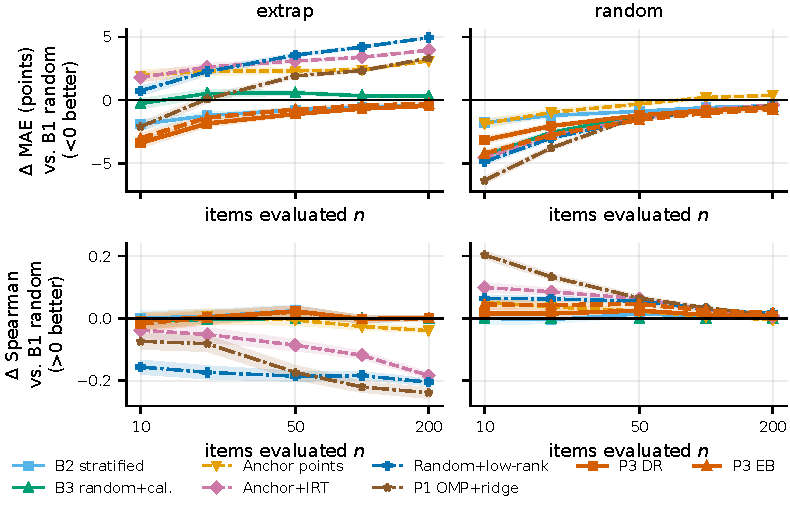
\includegraphics[width=\linewidth]{../figures/generated/fig_paired_diff.pdf}
\caption{Paired difference to the random subset mean (B1), macro-averaged over 13 benchmarks (95\% bootstrap bands). Top: MAE (negative is better); bottom: Spearman (positive is better). Left: extrapolation split; right: random split. $n{=}200$ covers 8 benchmarks.}
\label{fig:paired}
\end{figure}

\begin{figure}[h]
\centering
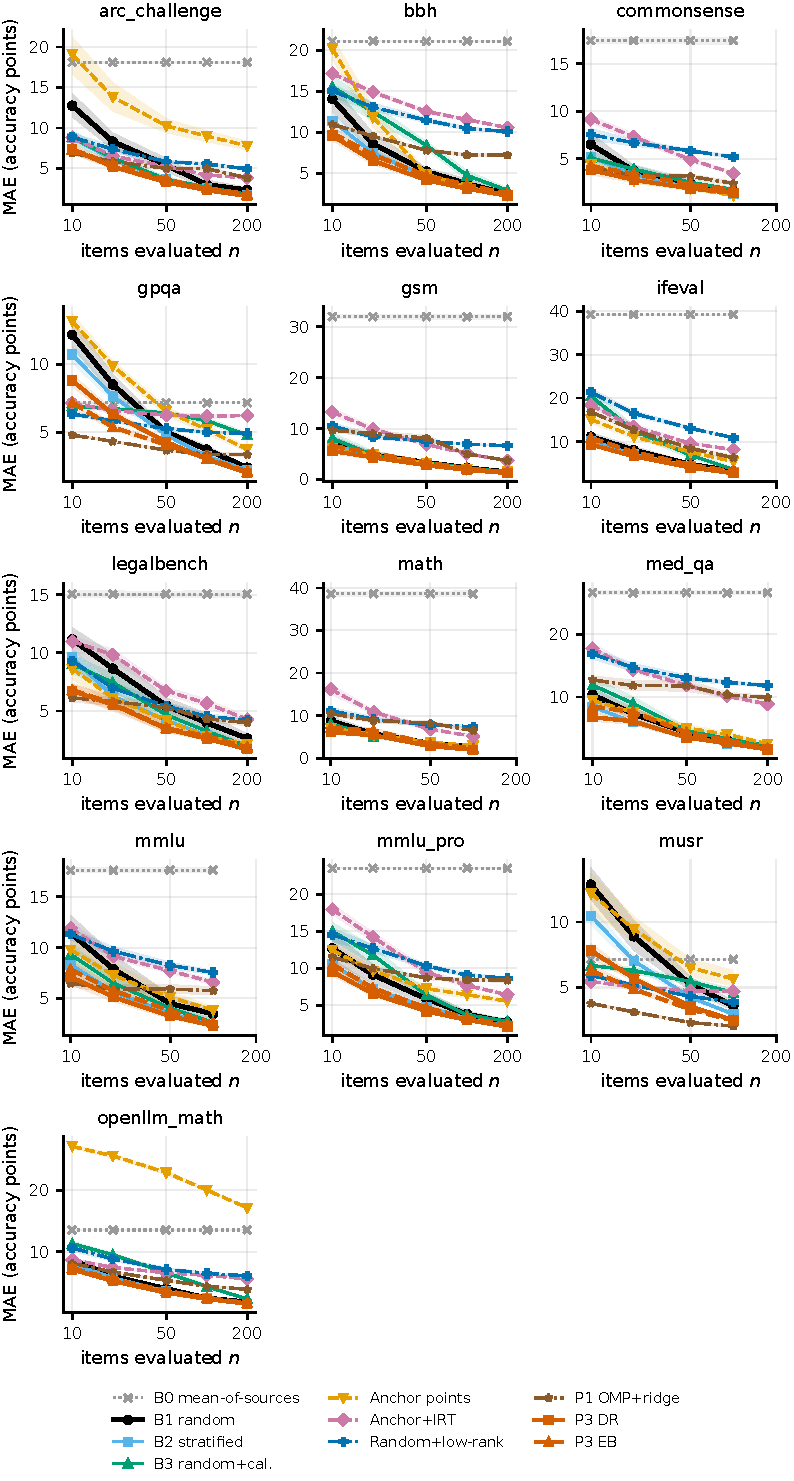
\includegraphics[width=0.8\linewidth]{../figures/generated/fig_mae_vs_n_extrap.pdf}
\caption{MAE against the number of items $n$, macro-average and per benchmark, extrapolation split, 95\% bands over repetitions. The same plot for the random split and the Spearman curves are in \texttt{figures/generated/}.}
\label{fig:curves}
\end{figure}

\begin{figure}[h]
\centering
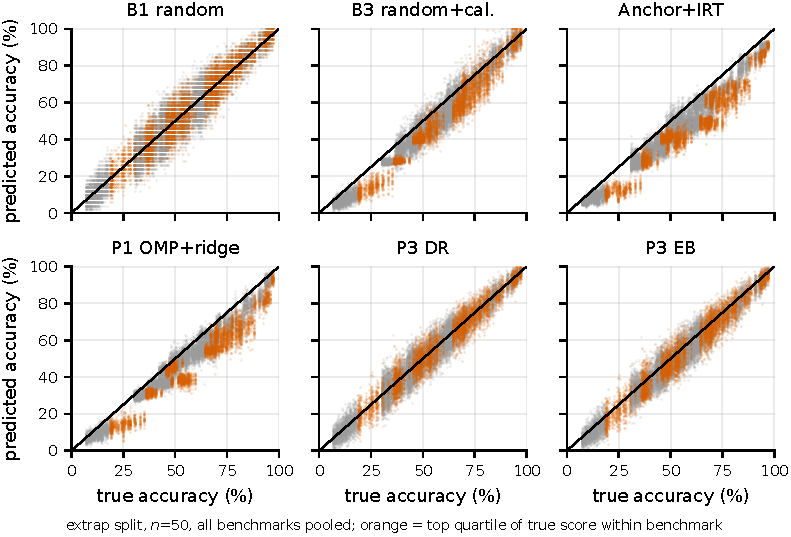
\includegraphics[width=0.8\linewidth]{../figures/generated/fig_scatter_extrap.pdf}
\caption{Predicted against true accuracy of target models, extrapolation split, $n{=}50$, all benchmarks pooled (orange: top quartile of true score within the benchmark).}
\label{fig:scatter}
\end{figure}

\begin{figure}[h]
\centering
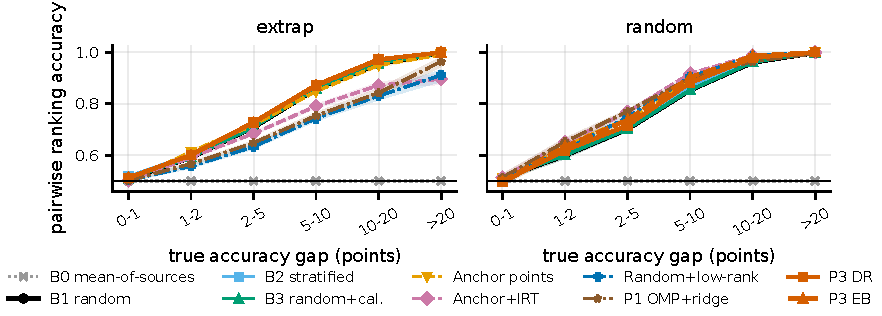
\includegraphics[width=0.9\linewidth]{../figures/generated/fig_pairwise_vs_gap.pdf}
\caption{Fraction of target-model pairs ordered correctly, by the true accuracy gap of the pair, $n{=}50$, macro-average over benchmarks.}
\label{fig:pairwise}
\end{figure}

\section{Further results}
\label{app:further}
\begin{table}[h]
\caption{Squared bias and variance of the prediction of a target model's accuracy over repetitions, in points$^2$, averaged over targets and benchmarks, $n{=}50$ (\texttt{paper/make\_tables.py} from \texttt{results/tables/tier1/q4\_bias\_variance.csv}). The squared bias of an unbiased design is not zero because it is estimated from a finite number of draws: $30$ on the extrapolation split, about $7.5$ on the random split (a model is a target in a quarter of the repetitions).}
\label{tab:q4}
\centering
{\scriptsize
\begin{tabular}{lrrrr}
\toprule
 & \multicolumn{2}{c}{random split} & \multicolumn{2}{c}{extrapolation} \\
\cmidrule(lr){2-3}\cmidrule(lr){4-5}
Method & bias$^2$ & variance & bias$^2$ & variance \\
\midrule
B0 mean of sources & 247.7 & 0.5 & 580.3 & 0.6 \\
B1 random & 5.1 & 29.9 & 1.2 & 32.2 \\
B2 stratified & 3.6 & 19.6 & 0.7 & 22.6 \\
B3 random + calibration & 5.6 & 13.5 & 25.7 & 13.4 \\
Anchor points & 13.7 & 18.9 & 109.3 & 23.2 \\
Anchor + IRT & 12.2 & 7.0 & 73.5 & 5.0 \\
Random + low-rank & 7.9 & 8.9 & 87.5 & 3.8 \\
P1 OMP + ridge & 9.2 & 18.3 & 57.6 & 7.3 \\
P3 DR (stratified + low-rank + correction) & 3.1 & 16.4 & 1.3 & 18.0 \\
P3 EB (shrunk correction) & 3.5 & 12.2 & 5.9 & 16.8 \\
\bottomrule
\end{tabular}}

\end{table}


\paragraph{Benchmark properties.}
Across the 13 benchmarks, the gain of P3 DR over B1 at $n{=}50$ (a negative MAE difference) is correlated with the spread of the item accuracies over source models (Spearman $-0.91$, bootstrap interval $[-0.99,-0.66]$ on the random split; $-0.82$, $[-0.95,-0.50]$ on the extrapolation split: more heterogeneous items, larger gain) and, positively, with the share of variance in the first singular component of the item matrix ($+0.62$ and $+0.65$; intervals exclude zero). The number of models, the number of items, the model-accuracy spread and the mean accuracy show no significant relation. This is descriptive: 13 benchmarks, nine properties examined per method without correction for multiplicity, and benchmarks that share models (\texttt{results/tables/tier1/q5\_benchmark\_properties.csv}).

\paragraph{Calibration of analytic intervals.}
As a by-product, we checked whether the nominal 95\% interval of a single model (finite-population standard error for B1, a Hajek residual standard error for the design-based estimators) covers the true score (Table~\ref{tab:coverage}). The pooled coverage is $0.86$ to $0.94$ and is below nominal at $n{=}20$ and on the random split (B1: $0.86$ at $n{=}20$ on the random split, $0.94$ at $n{=}100$ on the extrapolation split), so per-model analytic intervals are somewhat optimistic at small budgets. The intervals reported in this paper are bootstrap intervals over the study, not these.

\paragraph{All four metrics} (RMSE, Kendall and Spearman agree with MAE; Table~\ref{tab:metrics}).
\begin{table}[h]
\caption{Difference to B1 at $n{=}50$ in MAE, RMSE, Spearman and Kendall (macro-average over 13 benchmarks, 95\% two-level bootstrap intervals over repetitions and target models). Kendall's $\tau$ was bootstrapped over targets for seven methods only (dashes: not computed). Values from \texttt{results/tables/review/target\_bootstrap\_macro.csv}.}
\label{tab:metrics}\centering\resizebox{\linewidth}{!}{{\scriptsize\setlength{\tabcolsep}{3pt}
\begin{tabular}{lrrrr}
\toprule
Difference to B1 at $n{=}50$ & MAE (points) & RMSE (points) & Spearman & Kendall \\
\midrule
\multicolumn{5}{l}{\emph{random split}} \\
B2 stratified & -0.88\,{\tiny[-1.04,-0.73]} & -1.00\,{\tiny[-1.18,-0.83]} & +0.01\,{\tiny[+0.00,+0.03]} & +0.01\,{\tiny[+0.00,+0.03]} \\
B3 random + calibration & -1.23\,{\tiny[-1.36,-1.09]} & -1.44\,{\tiny[-1.56,-1.30]} & +0.00\,{\tiny[+0.00,+0.00]} & +0.00\,{\tiny[+0.00,+0.00]} \\
Anchor points & -0.30\,{\tiny[-0.50,-0.10]} & -0.35\,{\tiny[-0.57,-0.15]} & +0.02\,{\tiny[+0.01,+0.04]} & -- \\
Anchor + IRT & -1.44\,{\tiny[-1.60,-1.28]} & -1.54\,{\tiny[-1.75,-1.36]} & +0.06\,{\tiny[+0.05,+0.07]} & -- \\
Random + low-rank & -1.50\,{\tiny[-1.64,-1.35]} & -1.74\,{\tiny[-1.90,-1.57]} & +0.06\,{\tiny[+0.05,+0.06]} & +0.04\,{\tiny[+0.03,+0.05]} \\
P1 OMP + ridge & -1.27\,{\tiny[-1.45,-1.09]} & -1.17\,{\tiny[-1.45,-0.98]} & +0.07\,{\tiny[+0.05,+0.08]} & -- \\
Random + low-rank + correction & -1.13\,{\tiny[-1.26,-0.99]} & -1.28\,{\tiny[-1.42,-1.13]} & +0.02\,{\tiny[+0.01,+0.02]} & +0.00\,{\tiny[-0.00,+0.01]} \\
P3 DR & -1.20\,{\tiny[-1.36,-1.05]} & -1.37\,{\tiny[-1.54,-1.20]} & +0.02\,{\tiny[+0.01,+0.04]} & +0.01\,{\tiny[+0.00,+0.02]} \\
P3 EB & -1.56\,{\tiny[-1.72,-1.40]} & -1.81\,{\tiny[-1.97,-1.63]} & +0.05\,{\tiny[+0.04,+0.06]} & +0.04\,{\tiny[+0.02,+0.05]} \\
\multicolumn{5}{l}{\emph{extrapolation split}} \\
B2 stratified & -0.77\,{\tiny[-0.95,-0.61]} & -0.83\,{\tiny[-1.01,-0.65]} & +0.02\,{\tiny[+0.00,+0.05]} & +0.02\,{\tiny[+0.00,+0.04]} \\
B3 random + calibration & +0.58\,{\tiny[+0.38,+0.77]} & +0.39\,{\tiny[+0.20,+0.59]} & +0.00\,{\tiny[-0.00,+0.00]} & +0.00\,{\tiny[-0.00,+0.00]} \\
Anchor points & +2.31\,{\tiny[+2.11,+2.52]} & +3.07\,{\tiny[+2.85,+3.26]} & -0.00\,{\tiny[-0.03,+0.01]} & -- \\
Anchor + IRT & +3.10\,{\tiny[+2.91,+3.28]} & +2.94\,{\tiny[+2.75,+3.13]} & -0.09\,{\tiny[-0.11,-0.06]} & -- \\
Random + low-rank & +3.56\,{\tiny[+3.37,+3.74]} & +3.50\,{\tiny[+3.32,+3.69]} & -0.19\,{\tiny[-0.21,-0.16]} & -0.17\,{\tiny[-0.19,-0.15]} \\
P1 OMP + ridge & +1.91\,{\tiny[+1.71,+2.12]} & +1.98\,{\tiny[+1.77,+2.21]} & -0.17\,{\tiny[-0.20,-0.14]} & -- \\
Random + low-rank + correction & -0.99\,{\tiny[-1.14,-0.83]} & -1.07\,{\tiny[-1.24,-0.92]} & -0.00\,{\tiny[-0.01,+0.00]} & -0.02\,{\tiny[-0.03,-0.01]} \\
P3 DR & -1.10\,{\tiny[-1.27,-0.94]} & -1.21\,{\tiny[-1.39,-1.05]} & +0.02\,{\tiny[-0.00,+0.04]} & +0.00\,{\tiny[-0.02,+0.02]} \\
P3 EB & -0.74\,{\tiny[-0.92,-0.58]} & -0.85\,{\tiny[-1.03,-0.66]} & +0.02\,{\tiny[-0.00,+0.04]} & -0.00\,{\tiny[-0.02,+0.02]} \\
\bottomrule
\end{tabular}}
}
\end{table}

\paragraph{Tables of the further analyses} (organisation hold-out, selector$\times$estimator, number of source models, rank of the latent model, interval coverage; Section~\ref{sec:exp}).
\begin{table}[h]
\caption{Macro MAE (points) at $n{=}50$ on the four Open LLM Leaderboard benchmarks, 20 repetitions, for three kinds of split.}
\label{tab:family}\centering{\scriptsize
\begin{tabular}{lrrr}
\toprule
Method & random & organisation hold-out & extrapolation \\
\midrule
B1 random & 4.91 & 4.87 & 5.21 \\
B2 stratified & 4.18 & 4.20 & 4.61 \\
B3 random+calib. & 3.55 & 3.55 & 7.03 \\
Anchor points & 4.27 & 4.43 & 6.58 \\
Anchor+IRT & 2.95 & 3.06 & 9.47 \\
Random+low-rank & 2.78 & 2.88 & 10.04 \\
OMP+ridge & 1.95 & 2.20 & 7.16 \\
Random+low-rank+corr. & 3.76 & 3.76 & 4.30 \\
P3 DR & 3.72 & 3.73 & 4.18 \\
P3 EB & 3.06 & 3.09 & 4.52 \\
\bottomrule
\end{tabular}}

\end{table}
\begin{table}[h]
\caption{Macro MAE (points) of selector $\times$ estimator at $n{=}50$, 7 benchmarks, 20 repetitions. B1 is random + mean. Dashes: combination not run.}
\label{tab:factorial}\centering{\scriptsize\setlength{\tabcolsep}{3pt}
\begin{tabular}{lrrrrrrr}
\toprule
Selector $\backslash$ estimator & mean & calib. & ridge & IRT & low-rank & IRT+corr. & low-rank+corr. \\
\midrule
\multicolumn{8}{l}{\emph{random split}} \\
random & 4.82 & 3.68 & 3.22 & 3.64 & 3.21 & 3.91 & 3.73 \\
stratified & 3.97 & 3.47 & 3.12 & 3.49 & 3.14 & 3.74 & 3.64 \\
PPS & -- & 3.71 & 3.25 & 3.57 & 3.24 & 3.79 & 3.67 \\
anchor & -- & 3.42 & 2.96 & 3.32 & 3.08 & -- & -- \\
OMP & 8.53 & 3.01 & 3.52 & 3.27 & 2.86 & -- & -- \\
c-optimal & 14.91 & 3.01 & 3.04 & 3.78 & 2.98 & -- & -- \\
\multicolumn{8}{l}{\emph{extrapolation split}} \\
random & 4.65 & 5.82 & 8.69 & 9.65 & 9.87 & 3.99 & 3.91 \\
stratified & 4.04 & 5.39 & 8.94 & 9.42 & 9.84 & 3.90 & 3.72 \\
PPS & -- & 5.72 & 8.40 & 9.38 & 9.56 & 4.11 & 4.03 \\
anchor & -- & 6.00 & 8.76 & 9.19 & 9.92 & -- & -- \\
OMP & 13.25 & 5.45 & 7.76 & 8.48 & 9.63 & -- & -- \\
c-optimal & 30.71 & 11.45 & 11.73 & 10.77 & 11.43 & -- & -- \\
\bottomrule
\end{tabular}}

\end{table}
\begin{table}[h]
\caption{Macro MAE (points) at $n{=}50$ with 10, 20, 40 or all source models (7 benchmarks, 20 repetitions).}
\label{tab:ssize}\centering{\scriptsize\setlength{\tabcolsep}{3pt}
\begin{tabular}{lrrrrrrrr}
\toprule
 & \multicolumn{4}{c}{random split, $|\mathcal S|=$} & \multicolumn{4}{c}{extrapolation, $|\mathcal S|=$} \\
\cmidrule(lr){2-5}\cmidrule(lr){6-9}
Method & 10 & 20 & 40 & all & 10 & 20 & 40 & all \\
\midrule
B1 random & 4.82 & 4.82 & 4.82 & 4.79 & 4.65 & 4.65 & 4.65 & 4.71 \\
B2 stratified & 4.29 & 4.23 & 4.15 & 3.96 & 4.31 & 4.20 & 4.15 & 4.06 \\
Anchor+IRT & 8.08 & 5.42 & 4.08 & 3.33 & 19.39 & 14.77 & 11.29 & 9.19 \\
Random+low-rank & 5.38 & 4.43 & 3.64 & 3.18 & 14.24 & 12.76 & 11.06 & 9.85 \\
OMP+ridge & 5.50 & 4.47 & 4.10 & 3.45 & 13.62 & 11.14 & 9.65 & 7.78 \\
Random+low-rank+corr. & 4.24 & 4.02 & 3.84 & 3.72 & 4.51 & 4.31 & 4.01 & 3.86 \\
P3 DR & 4.15 & 4.00 & 3.87 & 3.63 & 4.26 & 4.19 & 3.87 & 3.75 \\
P3 EB & 3.94 & 3.69 & 3.46 & 3.18 & 4.83 & 4.78 & 4.33 & 4.22 \\
\bottomrule
\end{tabular}}

\end{table}
\begin{table}[h]
\caption{Macro MAE (points) at $n{=}50$ of the stratified design with a low-rank model of rank $k$ (5 benchmarks, 20 repetitions; $k{=}8$ is the frozen P3).}
\label{tab:rank}\centering{\scriptsize
\begin{tabular}{llrrrrr}
\toprule
 & stratified design with & $k{=}2$ & $k{=}4$ & $k{=}8$ & $k{=}16$ & $k{=}32$ \\
\midrule
random split & plain model & 3.33 & 3.24 & 3.24 & 3.32 & 3.62 \\
 & + correction (DR) & 3.74 & 3.68 & 3.61 & 3.53 & 3.55 \\
 & + shrunk correction (EB) & 3.25 & 3.22 & 3.21 & 3.25 & 3.42 \\
extrapolation split & plain model & 10.61 & 9.58 & 9.49 & 9.55 & 10.09 \\
 & + correction (DR) & 3.61 & 3.55 & 3.55 & 3.74 & 5.09 \\
 & + shrunk correction (EB) & 3.96 & 3.92 & 4.02 & 4.30 & 5.68 \\
\bottomrule
\end{tabular}}

\end{table}
\begin{table}[h]
\caption{Pooled coverage of the nominal 95\% analytic interval of single-model predictions (7 benchmarks, 20 repetitions).}
\label{tab:coverage}\centering{\scriptsize
\begin{tabular}{llrrr}
\toprule
split & $n$ & B1 (analytic) & random+low-rank+corr. & P3 DR \\
\midrule
extrap & 20 & 0.916 & 0.890 & 0.889 \\
extrap & 50 & 0.935 & 0.921 & 0.927 \\
extrap & 100 & 0.942 & 0.936 & 0.940 \\
random & 20 & 0.863 & 0.863 & 0.883 \\
random & 50 & 0.904 & 0.908 & 0.906 \\
random & 100 & 0.917 & 0.922 & 0.921 \\
\bottomrule
\end{tabular}}

\end{table}

\section{What was done and not done}
\label{app:honest}

\paragraph{Pilots and the freeze of P3.}
Before the design freeze, a handful of 2--4-seed trials on GPQA and MMLU-Pro (random and extrapolation splits, with the outer targets) were used to debug code and to decide the list of candidate pipelines; they are not part of any reported number. The choice of P3 was made afterwards by the lowest mean MAE rank in an inner cross-validation of IFEval, GSM8K and MMLU-Pro that uses source models only (8 repetitions, budgets 10--200; \texttt{results/freeze/}). During debugging, IRT dimensions 1, 4 and 8 were tried once on GPQA, BBH and MMLU-Pro (random split, one seed); dimension 8 looked slightly better on two of three and 4 was kept.

\paragraph{Forbidden-content disclosure.}
The task forbids reading the published paper on this question. While looking for the row-to-model correspondence of the HELM files, the implementer of the experiments opened the README of the data repository (about 80 lines, as directed by the task's data description) and a file list. The README's opening lines state, in two sentences, the conclusion of the paper that accompanies the repository: that methods interpolate among similar models, and that all but random sampling and one doubly-robust estimator fail for very different targets. The paper itself, the \texttt{benchpred} code and later citing works were not opened. The model-assisted difference estimator, the extrapolation split and all candidate designs were implemented and the design-freeze runs launched before the README was opened; the ranking that froze P3 was computed after. The README did not add a candidate or change the selection rule, but independence is partial. The writer of this paper and the context position read only the abstracts of the starter literature, which the task allows.

\paragraph{Not done at the time of writing.}
Active Evaluation Acquisition, the metabench GAM predictor, gp-IRT and the Pacchiardi assessor are not implemented; the \texttt{benchpred} package was not run. The organisation hold-out exists for the four Open LLM Leaderboard benchmarks only; the selector$\times$estimator, source-size and rank analyses cover 5--7 benchmarks and 20 repetitions; a hold-out of model families by size or release date was not run.

\paragraph{Reproduction and compute.}
Environment, data download commands, seeds, commands and run times are in \texttt{REPRODUCE.md}; scripts: \texttt{code/} (analysis; Tier 1 took 1.9 hours of single-job time on 2 CPU cores per job as logged in \texttt{results/tables/tier1/timing\_by\_shard.csv}), \texttt{figures/} (figures and the data table), \texttt{paper/make\_tables.py} (Tables~\ref{tab:macro} and~\ref{tab:q4}). The paper builds with \texttt{paper/build.sh}.


\newpage
\section*{NeurIPS Paper Checklist}




\begin{enumerate}

\item {\bf Claims}
    \item[] Question: Do the main claims made in the abstract and introduction accurately reflect the paper's contributions and scope?
    \item[] Answer: \answerYes{} % Replace by \answerYes{}, \answerNo{}, or \answerNA{}.
    \item[] Justification: The abstract and introduction state the questions Q1--Q4 and the findings (source-model information helps on random splits, model-based predictors lose under extrapolation, a design-based residual correction, not stratification, is what makes them robust, at a small gain over random sampling and a cost when targets resemble the sources); they are supported by Section~5 and bounded by Section~6.

\item {\bf Limitations}
    \item[] Question: Does the paper discuss the limitations of the work performed by the authors?
    \item[] Answer: \answerYes{} % Replace by \answerYes{}, \answerNo{}, or \answerNA{}.
    \item[] Justification: Section~6 lists the limitations: re-implemented methods, fixed hyperparameters, 20--107 target models, shared models across benchmarks, one kind of shift, budget cap, partial independence of the P3 design, further analyses on 4--7 benchmarks and no family hold-out by size or date.

\item {\bf Theory assumptions and proofs}
    \item[] Question: For each theoretical result, does the paper provide the full set of assumptions and a complete (and correct) proof?
    \item[] Answer: \answerNA{} % Replace by \answerYes{}, \answerNo{}, or \answerNA{}.
    \item[] Justification: The paper states no theorem; the difference estimator used in P3 is a standard survey-sampling estimator and no new proof is claimed.

    \item {\bf Experimental result reproducibility}
    \item[] Question: Does the paper fully disclose all the information needed to reproduce the main experimental results of the paper to the extent that it affects the main claims and/or conclusions of the paper (regardless of whether the code and data are provided or not)?
    \item[] Answer: \answerYes{} % Replace by \answerYes{}, \answerNo{}, or \answerNA{}.
    \item[] Justification: Sections~3--5 and Appendices~A--B give the data version, split definitions, methods, hyperparameters, metrics and seeds; \texttt{REPRODUCE.md} gives commands and run times.


\item {\bf Open access to data and code}
    \item[] Question: Does the paper provide open access to the data and code, with sufficient instructions to faithfully reproduce the main experimental results, as described in supplemental material?
    \item[] Answer: \answerYes{} % Replace by \answerYes{}, \answerNo{}, or \answerNA{}.
    \item[] Justification: All data are public at a pinned commit; code, per-prediction results and reproduction instructions are delivered with the paper (\texttt{code/}, \texttt{results/}, \texttt{REPRODUCE.md}, \texttt{figures/}) and referred to as supplementary material.


\item {\bf Experimental setting/details}
    \item[] Question: Does the paper specify all the training and test details (e.g., data splits, hyperparameters, how they were chosen, type of optimizer) necessary to understand the results?
    \item[] Answer: \answerYes{} % Replace by \answerYes{}, \answerNo{}, or \answerNA{}.
    \item[] Justification: Section~5 and Appendix~A state the splits, numbers of source and target models, budgets, seeds and how hyperparameters were set (fixed a priori, or by cross-validation inside the source models only).

\item {\bf Experiment statistical significance}
    \item[] Question: Does the paper report error bars suitably and correctly defined or other appropriate information about the statistical significance of the experiments?
    \item[] Answer: \answerYes{} % Replace by \answerYes{}, \answerNo{}, or \answerNA{}.
    \item[] Justification: Tables and figures report 95\% percentile-bootstrap intervals over 30 repetitions (20 in the further analyses) and paired differences to the baseline; for the headline paired differences a two-level bootstrap over repetitions and target models is also reported (Section~5); intervals treat the 13 benchmarks as fixed and they are not independent (stated).

\item {\bf Experiments compute resources}
    \item[] Question: For each experiment, does the paper provide sufficient information on the computer resources (type of compute workers, memory, time of execution) needed to reproduce the experiments?
    \item[] Answer: \answerYes{} % Replace by \answerYes{}, \answerNo{}, or \answerNA{}.
    \item[] Justification: Appendix~B and \texttt{REPRODUCE.md} report CPU-only runs on 2 cores per job and measured times (1.9 hours of single-job time for the main run); memory per job is not reported.
    
\item {\bf Code of ethics}
    \item[] Question: Does the research conducted in the paper conform, in every respect, with the NeurIPS Code of Ethics \url{https://neurips.cc/public/EthicsGuidelines}?
    \item[] Answer: \answerYes{} % Replace by \answerYes{}, \answerNo{}, or \answerNA{}.
    \item[] Justification: The work uses only public benchmark score matrices and involves no human subjects; it follows the Code of Ethics, including honest reporting of failed or partial work.


\item {\bf Broader impacts}
    \item[] Question: Does the paper discuss both potential positive societal impacts and negative societal impacts of the work performed?
    \item[] Answer: \answerYes{} % Replace by \answerYes{}, \answerNo{}, or \answerNA{}.
    \item[] Justification: Section~6 (broader impact) discusses cheaper evaluation against the risks of over-trusting few-item estimates, misranking close models and gaming the subset.
    
\item {\bf Safeguards}
    \item[] Question: Does the paper describe safeguards that have been put in place for responsible release of data or models that have a high risk for misuse (e.g., pre-trained language models, image generators, or scraped datasets)?
    \item[] Answer: \answerNA{} % Replace by \answerYes{}, \answerNo{}, or \answerNA{}.
    \item[] Justification: No model or dataset with a high risk of misuse is released.

\item {\bf Licenses for existing assets}
    \item[] Question: Are the creators or original owners of assets (e.g., code, data, models), used in the paper, properly credited and are the license and terms of use explicitly mentioned and properly respected?
    \item[] Answer: \answerYes{} % Replace by \answerYes{}, \answerNo{}, or \answerNA{}.
    \item[] Justification: The score matrices are from the benchmark-prediction repository at a pinned commit (MIT licence, as stated by the task description), derived from the Open LLM Leaderboard and HELM (Apache-2.0); the upstream leaderboard data card declares no licence and we have not verified its terms further (Appendix~A, Section~3). The re-implemented methods are cited.

\item {\bf New assets}
    \item[] Question: Are new assets introduced in the paper well documented and is the documentation provided alongside the assets?
    \item[] Answer: \answerYes{} % Replace by \answerYes{}, \answerNo{}, or \answerNA{}.
    \item[] Justification: The released code and result tables are new assets, documented in \texttt{REPRODUCE.md}; no new dataset is introduced.

\item {\bf Crowdsourcing and research with human subjects}
    \item[] Question: For crowdsourcing experiments and research with human subjects, does the paper include the full text of instructions given to participants and screenshots, if applicable, as well as details about compensation (if any)? 
    \item[] Answer: \answerNA{} % Replace by \answerYes{}, \answerNo{}, or \answerNA{}.
    \item[] Justification: No crowdsourcing or human-subject research.

\item {\bf Institutional review board (IRB) approvals or equivalent for research with human subjects}
    \item[] Question: Does the paper describe potential risks incurred by study participants, whether such risks were disclosed to the subjects, and whether Institutional Review Board (IRB) approvals (or an equivalent approval/review based on the requirements of your country or institution) were obtained?
    \item[] Answer: \answerNA{} % Replace by \answerYes{}, \answerNo{}, or \answerNA{}.
    \item[] Justification: No human subjects, so no IRB approval applies.

\item {\bf Declaration of LLM usage}
    \item[] Question: Does the paper describe the usage of LLMs if it is an important, original, or non-standard component of the core methods in this research? Note that if the LLM is used only for writing, editing, or formatting purposes and does \emph{not} impact the core methodology, scientific rigor, or originality of the research, declaration is not required.
    %this research? 
    \item[] Answer: \answerYes{} % Replace by \answerYes{}, \answerNo{}, or \answerNA{}.
    \item[] Justification: Section~6 (use of LLM agents) states that the whole study was carried out by LLM-based agents under human-set objectives; the methods themselves use no LLM.

\end{enumerate}

\end{document}
